\documentclass[11pt,a4paper]{article}
\usepackage[margin=2.2cm]{geometry}
\usepackage{graphicx}
\usepackage{booktabs}
\usepackage{amsmath}
\usepackage{siunitx}
\usepackage{caption}
\usepackage{subcaption}
\usepackage[hidelinks]{hyperref}
\usepackage{xcolor}

\title{Latent-Diffusion Compression Trade-off Study on 21\,cm Fields\\
       \large 4 compression ratios (2$\times$/4$\times$/8$\times$/16$\times$) on the test set}
\author{Chenxi He (ch2067@cam.ac.uk)}
\date{\today}

\newcommand{\Mpc}{\mathrm{cMpc}^{-1}}
\newcommand{\relMSE}{\text{rel\_MSE}}
\newcommand{\relMSEf}{\text{rel\_MSE}_{\rm fluct}}

\begin{document}
\maketitle

\begin{abstract}
We train four latent-diffusion models (LDM) that share the same U-Net backbone and
conditioning stack but differ only in the compression ratio of the frozen VAE that
supplies the latent space --- 2$\times$, 4$\times$, 8$\times$ and 16$\times$
(latent-channel dimensions 32, 16, 8, 4 respectively).  All four chains are trained
for 124 epochs on the same multi-redshift ($z\!\in\![7,13]$, $z\!=\!10$ dominant)
data and evaluated on 130 held-out test cubes ($256^3$ voxels, Hann-window tiled
from $64^3$ patches).  We report per-cube pixel MSE, per-$k$ power-spectrum ratios,
equilateral bispectrum, Fourier cross-coherence, pixel PDF, redshift dependence and
inference wall-clock.  The main finding is that pixel MSE ranks the chains
misleadingly (4$\times$ has the lowest median $\relMSE$ because blurred output
regresses to the mean), whereas power-spectrum-based statistics unambiguously
identify \textbf{the 2$\times$ chain as the only paper-grade candidate}.
\end{abstract}

\section{Setup}
\label{sec:setup}

Test cubes are drawn from the \texttt{varying\_astro} suite, with $\sim\!100$
cubes at $z\!=\!10$ (the training-dominant redshift) and $\sim\!10$ cubes at each
of $z\!\in\!\{7,8,9,11\}$.  Each cube is generated tile-by-tile from $64^3$ patches
with 50\,\% Hann-window overlap; sampling uses Heun-order EDM with 30 steps.
Compression ratio $C\!=\!64/n_\mathrm{lat}$ where $n_\mathrm{lat}$ is the number of
latent channels (spatial dimensions are fixed at $16^3$ per patch).

\begin{table}[ht]
\centering
\caption{Overall test-set summary (median across 130 cubes; last row is inference
wall-clock per $256^3$ cube).  ``bias'' $=\sigma_\mathrm{true}/\sigma_\mathrm{gen}-1$:
positive means the generated field is under-variance (too blurry).}
\label{tab:summary}
\begin{tabular}{lcccc}
\toprule
Chain               & 2$\times$        & 4$\times$        & 8$\times$        & 16$\times$       \\
\midrule
median $\relMSE_{\rm fluct}$ & \textbf{0.521}   & 0.514            & 0.639            & 0.651            \\
median bias         & \textbf{+0.053}  & +0.283           & +0.427           & +0.490           \\
PS ratio $k\!<\!0.15$   & \textbf{0.96}& 0.73             & 0.77             & 0.89             \\
PS ratio $k\!\in[0.15,0.35]$ & \textbf{1.02}& 0.73        & 0.70             & 0.76             \\
PS ratio $k\!>\!0.35$   & \textbf{0.87}& 0.53             & 0.39             & 0.33             \\
mean gen time / cube    & 110\,s       & 110\,s           & 110\,s           & 110\,s           \\
\bottomrule
\end{tabular}
\end{table}

\section{Why pixel MSE is misleading}
\label{sec:mse-trap}

We initially used the naive normalisation
$\text{rel\_MSE}_{\rm raw}=\sum(t-g)^2/\sum t^2$.  This is severely biased for
21\,cm fields.  Concrete example (cube \#33 at $z\!=\!10$, 2$\times$ chain):
true $\bar t\!=\!+1.45$, $\sigma_t\!=\!0.18$; gen $\bar g\!=\!+1.17$,
$\sigma_g\!=\!0.23$.  The denominator
$\sum t^2 \propto \bar t^2 + \sigma_t^2 \approx 2.13$ is dominated by the
$\bar t^2\!\approx\!2.1$ DC term, so a generated field that is grossly wrong in
fluctuations still gets $\text{rel\_MSE}_{\rm raw}\!=\!0.063$ purely because the
truth has a nonzero mean.  Subtracting each cube's mean first,
$\relMSEf=\sum(t-\bar t-(g-\bar g))^2/\sum(t-\bar t)^2$,
gives the physically meaningful ratio and, for this same cube, jumps to
$\relMSEf\!=\!1.74$ --- worse than the trivial ``predict a constant'' baseline.
We therefore use $\relMSEf$ throughout this report.

\begin{figure}[hb]
\centering
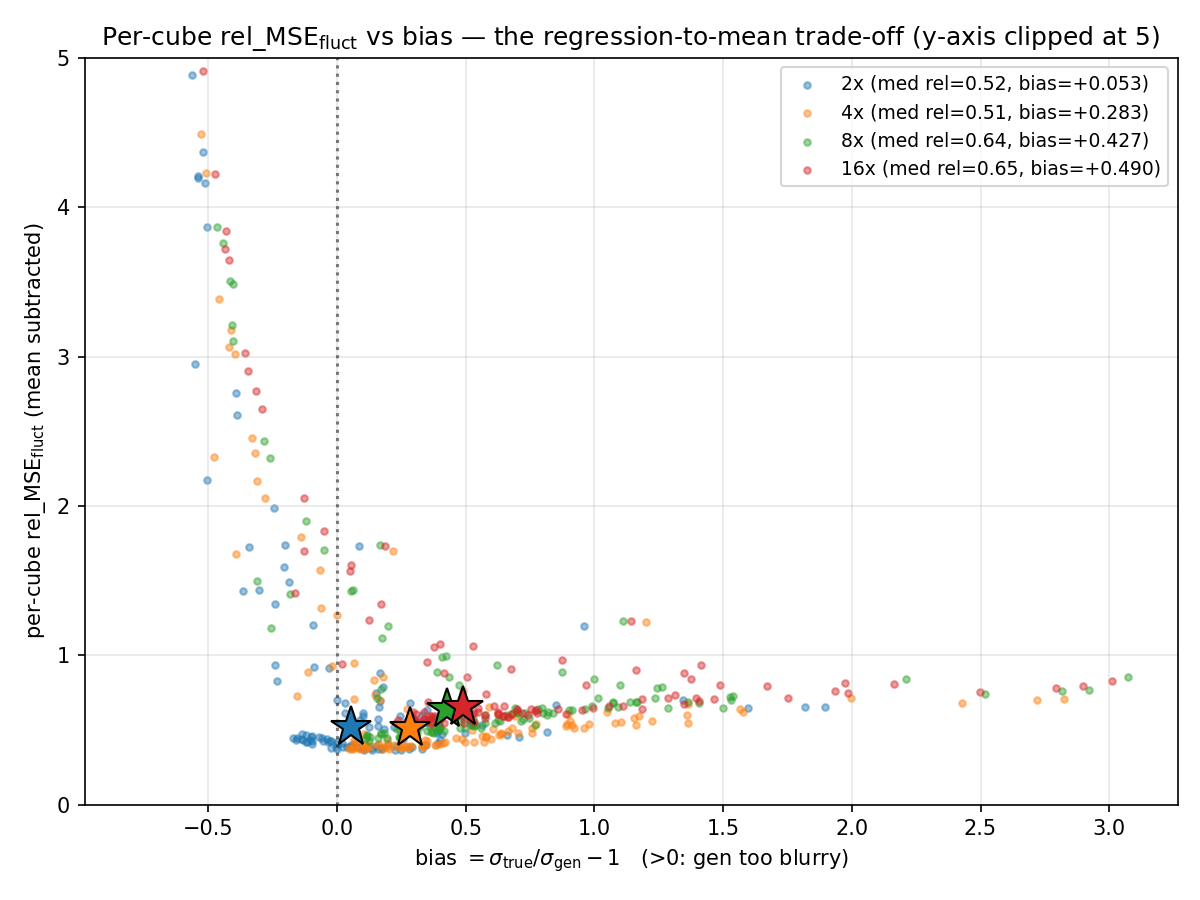
\includegraphics[width=0.95\linewidth]{figures/3_mse_bias_scatter.png}
\caption{Per-cube $\relMSEf$ (mean-subtracted) vs.\ bias, coloured by chain.
Stars mark the median per chain.  On this fair metric 2$\times$ (blue) and
4$\times$ (orange) are nearly tied in median $\relMSEf$; 2$\times$ wins
decisively on bias --- its cloud sits at $x\!\approx\!0$ while
4$\times$/8$\times$/16$\times$ drift progressively to the right (positive bias
$\Leftrightarrow$ under-variance).  The regression-to-the-mean trade-off is
still visible: chains with higher bias populate the low-$\relMSEf$ high-bias
region.  Y-axis clipped at 5 for readability; a handful of $z\!=\!7$ outliers
extend beyond.}
\label{fig:mse-bias}
\end{figure}

The takeaway: pixel MSE alone cannot rank the chains; you need to combine it
with the bias / power-spectrum diagnostics below.  On $\relMSEf$ + bias
jointly, 2$\times$ dominates.

\section{Power spectrum}
\label{sec:ps}

The power spectrum $P(k)$ is the primary statistic used to compare 21\,cm
predictions with observations.  We compute $P(k)$ in 20 log-spaced $k$-bins
between $k\!=\!0.05\,\Mpc$ and $k\!=\!0.95 k_{\rm nyq}$
(with $L_{\rm pix}\!=\!3\,\mathrm{cMpc}$, $k_{\rm nyq}\!=\!\pi/L_{\rm pix}$).

\begin{figure}[ht]
\centering
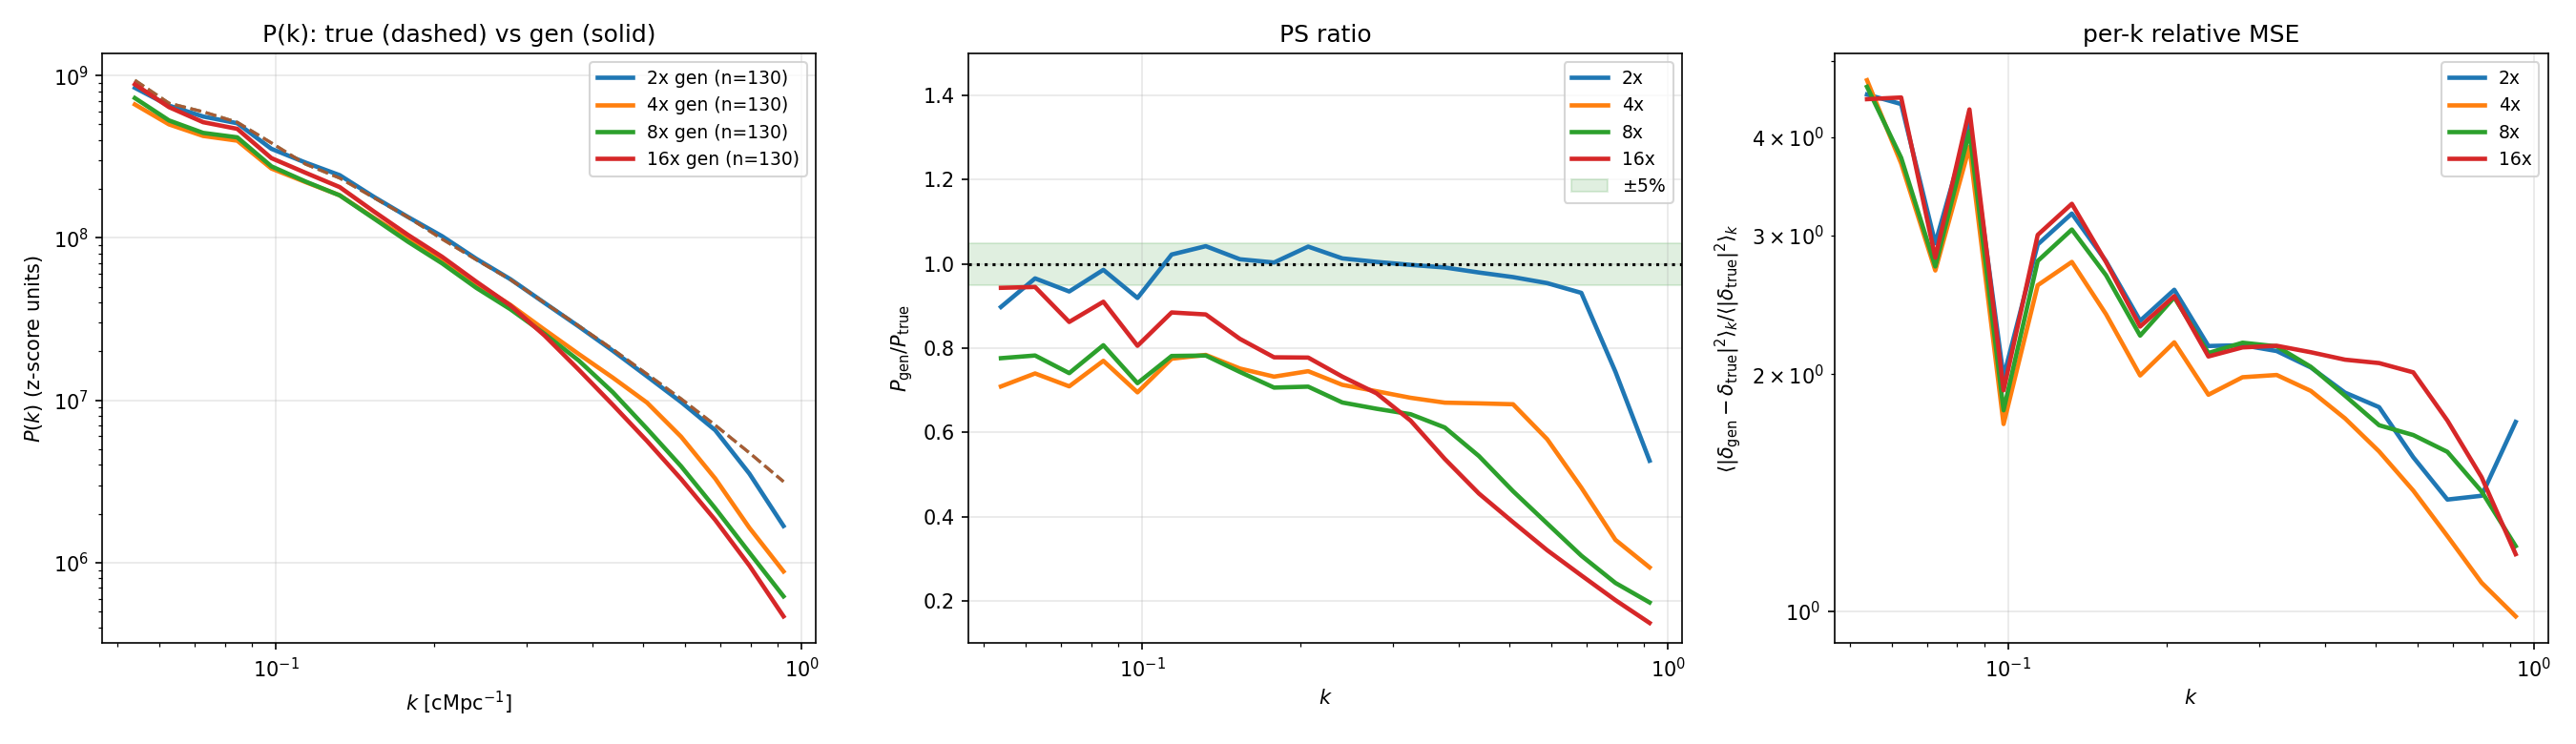
\includegraphics[width=\linewidth]{figures/1_ps_overview.png}
\caption{Left: mean $P(k)$ across 130 test cubes; dashed lines are the true
field, solid the generated field.  Middle: $P_\mathrm{gen}/P_\mathrm{true}$ ratio;
green band marks $[0.95,1.05]$ ($\pm 5\%$).  Right: per-$k$ relative MSE.  The
2$\times$ chain (blue) is the only one whose PS ratio stays inside or close to
the $\pm 5\%$ band across nearly two decades of $k$; higher-compression chains
lose $\sim\!25\,\%$ of the mid-$k$ power and up to $\sim\!70\,\%$ of the
Nyquist-scale power.}
\label{fig:ps-overview}
\end{figure}

\begin{figure}[ht]
\centering
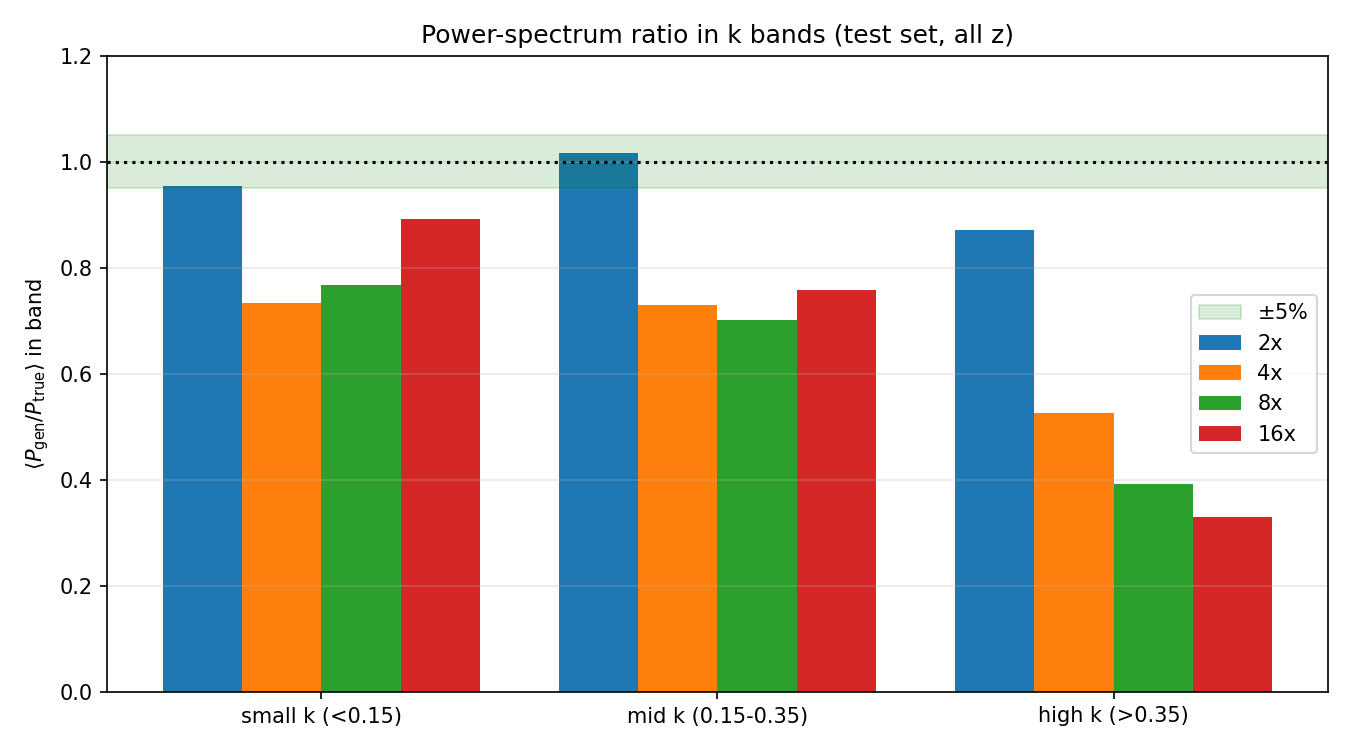
\includegraphics[width=0.75\linewidth]{figures/2_ps_ratio_bands.png}
\caption{Band-averaged PS ratios grouped by scale.  The 2$\times$ chain is the
only one that satisfies the $[0.95,1.05]$ paper grade at small and mid $k$; at
high $k$ ($k>0.35\,\Mpc$) all chains lose power because a single $64^3$ patch
cannot reproduce sub-tile structure, but the 2$\times$ chain still retains
87\,\% of the power there.  4$\times$/8$\times$/16$\times$ are systematically
deficient at every scale.}
\label{fig:ps-bands}
\end{figure}

\section{Higher-order statistics}
\label{sec:hos}

The 21\,cm field is markedly non-Gaussian; matching $P(k)$ alone is insufficient.
We check the bispectrum, the Fourier cross-coherence with the truth, and the
pixel PDF.

\begin{figure}[ht]
\centering
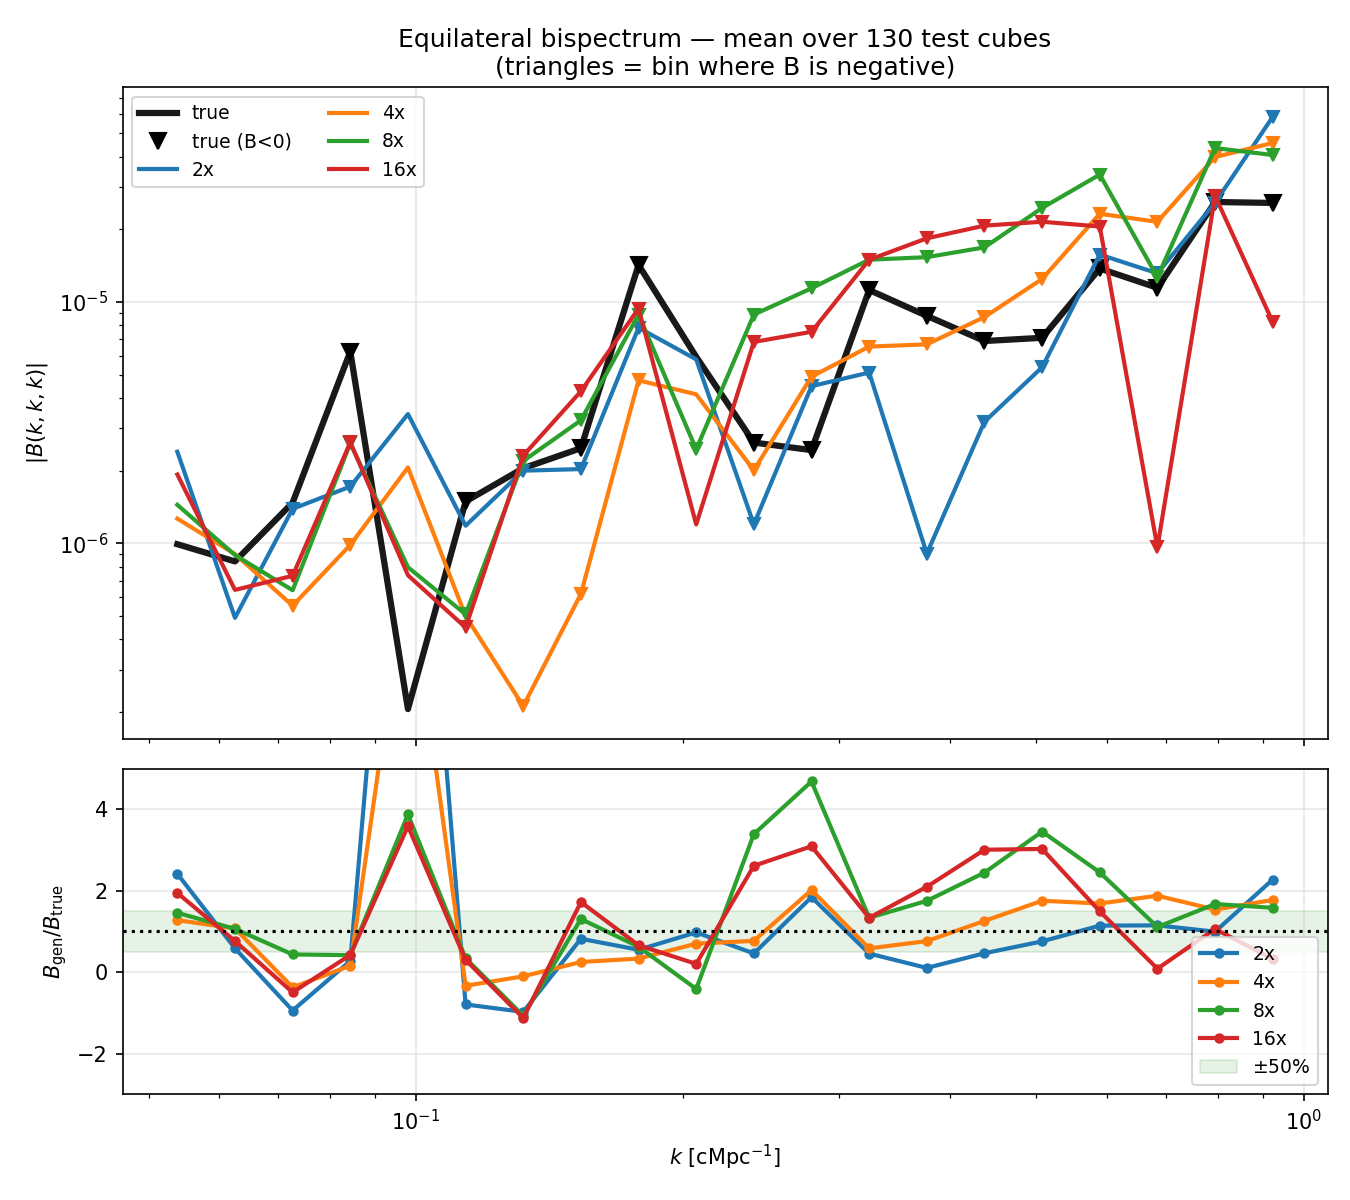
\includegraphics[width=0.85\linewidth]{figures/6_bispec_equilateral.png}
\caption{Equilateral bispectrum $B(k,k,k)$.  Because $B$ is a signed
quantity that fluctuates in sign across cubes, the 130-cube mean is inherently
noisy; triangles mark bins where the sign is negative.  The lower panel plots the
signed ratio $B_\mathrm{gen}/B_\mathrm{true}$.  2$\times$ is the only chain whose
ratio stays inside $\pm50\,\%$ (green band) at small and mid $k$; higher
compression amplifies the bispectrum by factors of 2--4 at $k\!>\!0.3\,\Mpc$,
indicating exaggerated non-Gaussianity from the diffusion sampling noise
leaking into the decoded output.}
\label{fig:bispec}
\end{figure}

\begin{figure}[ht]
\centering
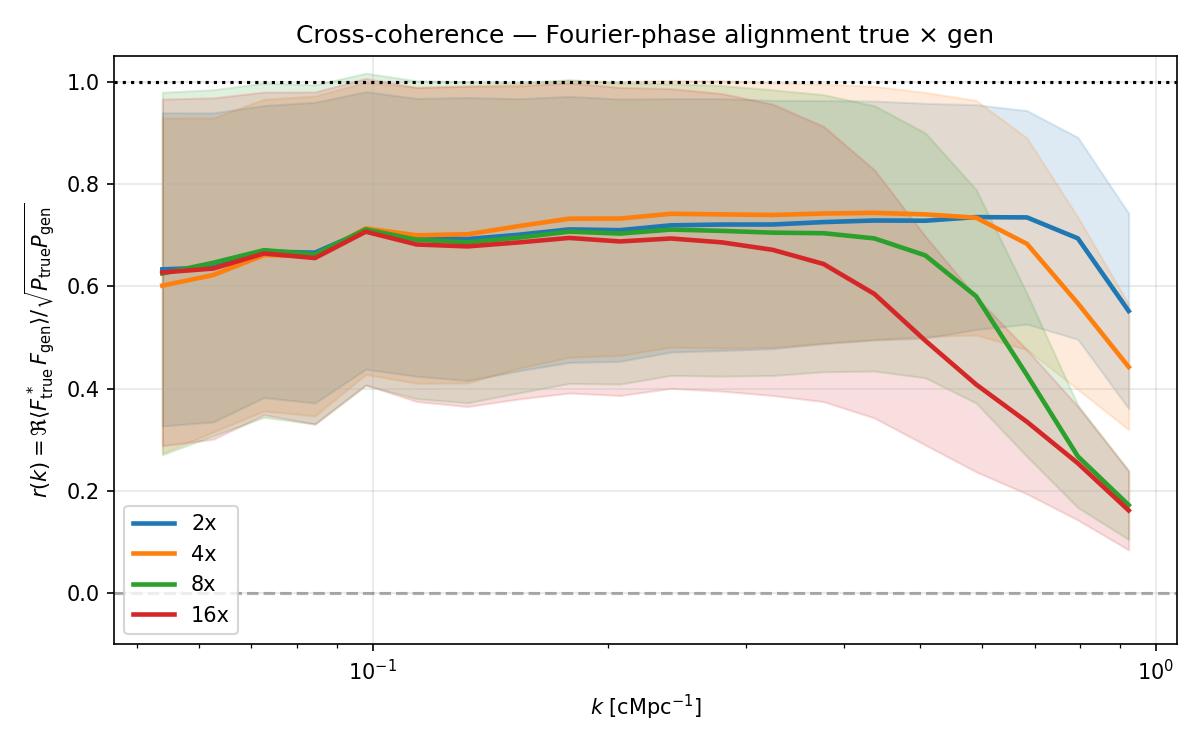
\includegraphics[width=0.7\linewidth]{figures/7_cross_coherence.png}
\caption{Cross-coherence
$r(k)=\Re\langle F^\ast_\mathrm{true} F_\mathrm{gen}\rangle
       / \sqrt{P_\mathrm{true}P_\mathrm{gen}}$, which measures how well the
Fourier phases of the generated field align with the truth ($r\!=\!1$ perfect,
$r\!=\!0$ decorrelated).  All chains achieve $r\!\approx\!0.7$ up to
$k\!\approx\!0.3\,\Mpc$ --- phase alignment is not the bottleneck --- but the
2$\times$ chain preserves coherence to noticeably higher $k$ than 8$\times$ or
16$\times$.  Shaded bands are the $\pm1\sigma$ scatter across cubes.}
\label{fig:xcoh}
\end{figure}

\begin{figure}[ht]
\centering
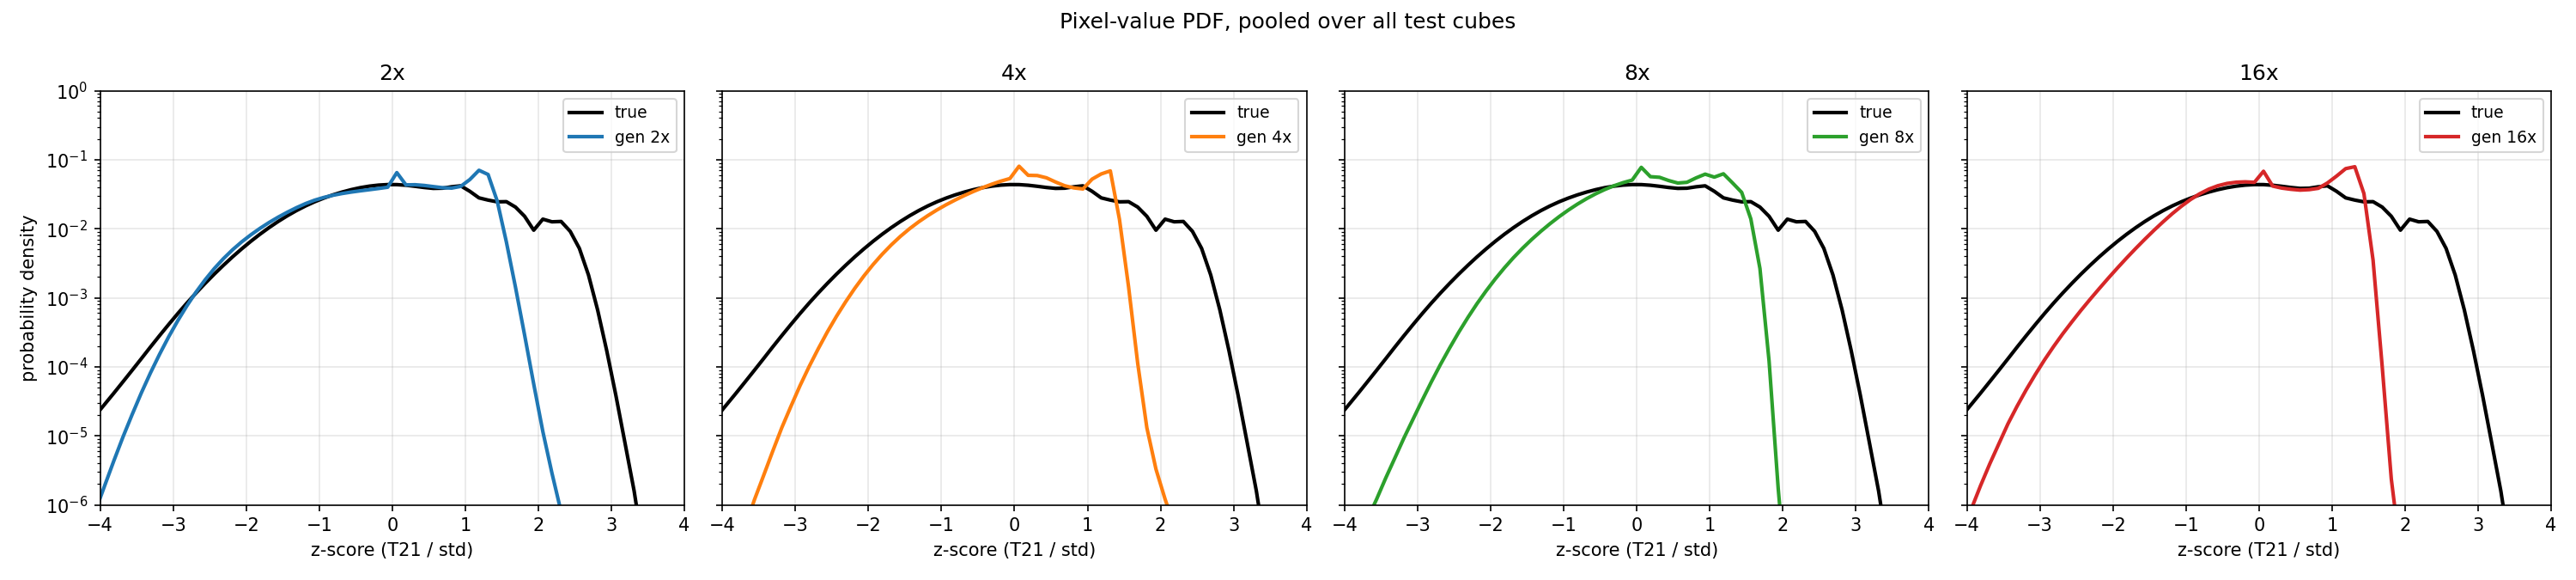
\includegraphics[width=\linewidth]{figures/8_pixel_pdf.png}
\caption{Voxel-value PDF pooled over all 130 test cubes, one panel per chain.
Black is the true distribution; coloured is the generated one.  All four chains
reproduce the peak location and the left tail (cold, absorption side) reasonably
well, but only 2$\times$ approximately captures the right tail (bright, emission
side, $z\!\ge\!1$).  Higher-compression chains truncate the right tail
progressively earlier, consistent with the variance deficit and the missing
high-$k$ power seen in Fig.~\ref{fig:ps-overview}.}
\label{fig:pdf}
\end{figure}

\section{Redshift dependence}
\label{sec:zdep}

The training set is $z\!=\!10$-heavy, so we expect performance to degrade
away from that redshift.  Figures \ref{fig:perz} and \ref{fig:perz-bar} confirm
this: $z\!=\!10$ has the smallest bias for every chain, and the away-from-training
redshifts inherit the compression penalty in variance deficit.

\begin{figure}[ht]
\centering
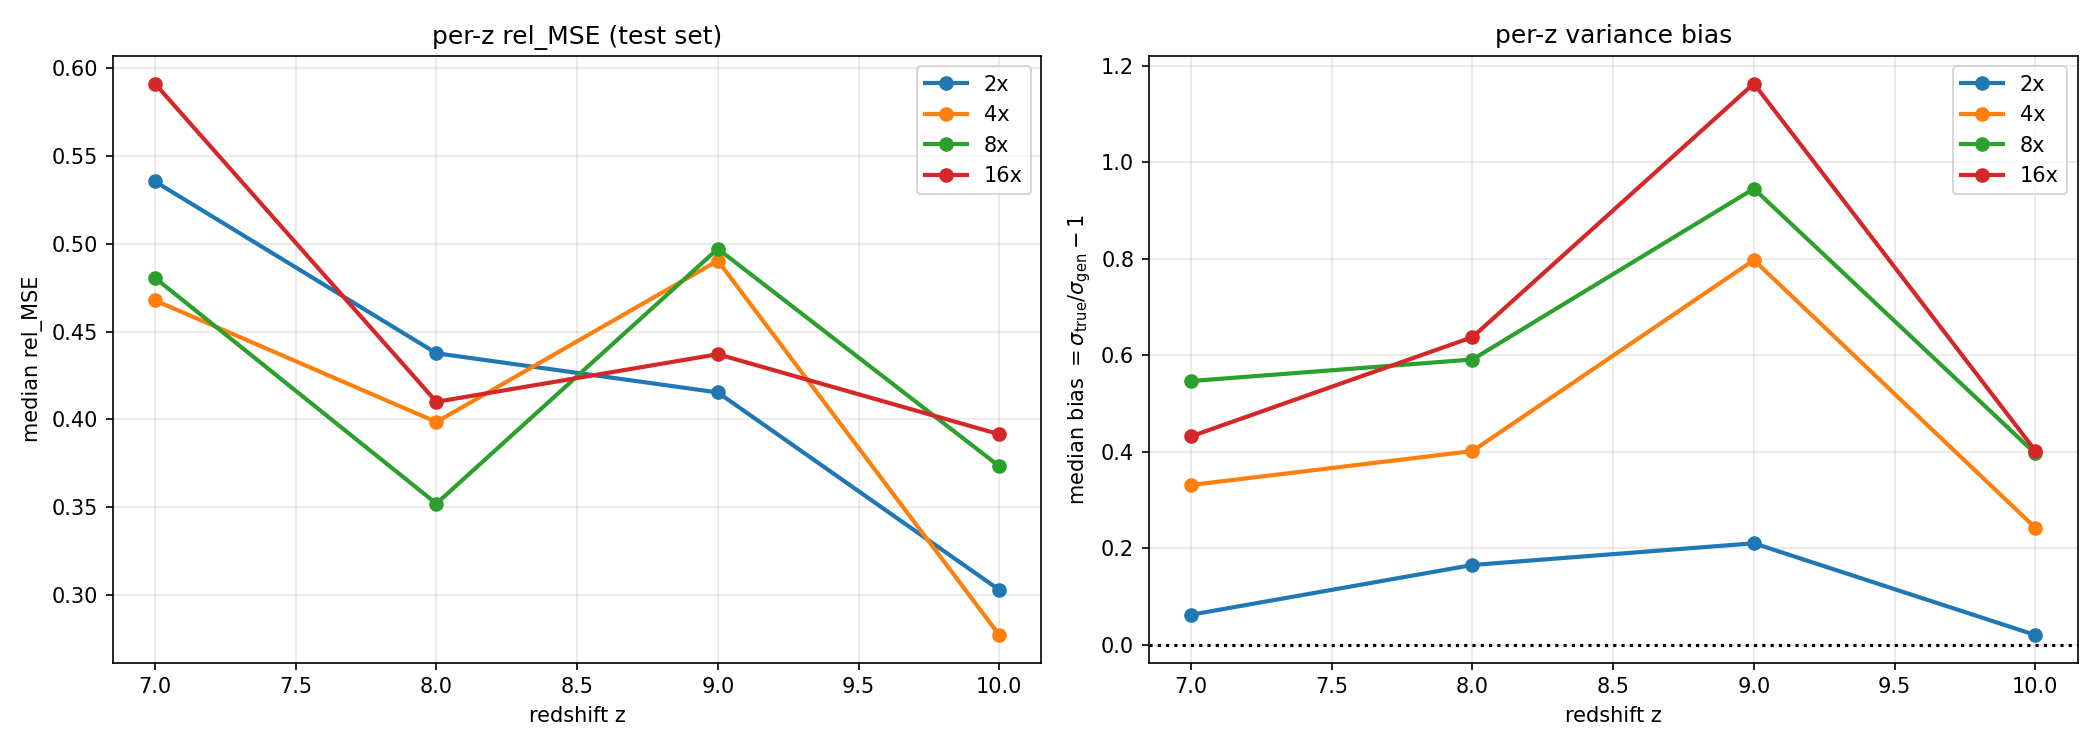
\includegraphics[width=\linewidth]{figures/4_per_z_summary.png}
\caption{Left: median per-cube $\relMSE$ vs.\ redshift.  Right: median bias vs.\
redshift (dotted line at bias $=0$ marks perfect variance match).  The 2$\times$
chain (blue) is nearly unbiased at every $z$; the higher-compression chains have
$\sim\!0.4\text{--}1.2$ bias at $z\!\in\!\{7,8,9\}$, i.e.\ the generated field
undershoots the true $\sigma$ by 40--55\,\%.}
\label{fig:perz}
\end{figure}

\begin{figure}[ht]
\centering
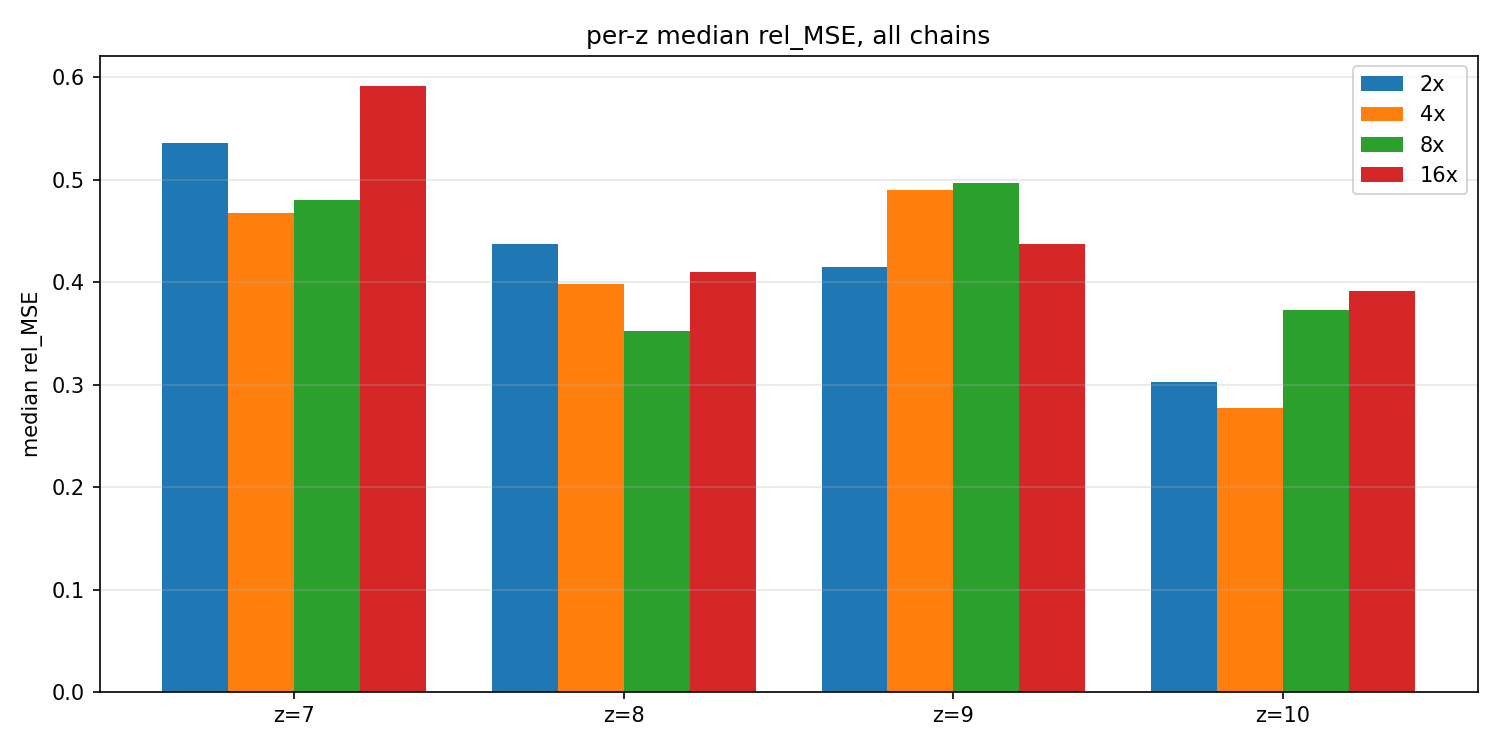
\includegraphics[width=0.85\linewidth]{figures/11_per_z_bars.png}
\caption{Same rel\_MSE data as Fig.~\ref{fig:perz} left, shown as a grouped bar
chart for easier visual ranking within each redshift.}
\label{fig:perz-bar}
\end{figure}

\section{Astro-parameter dependence}
\label{sec:corner}

\begin{figure}[ht]
\centering
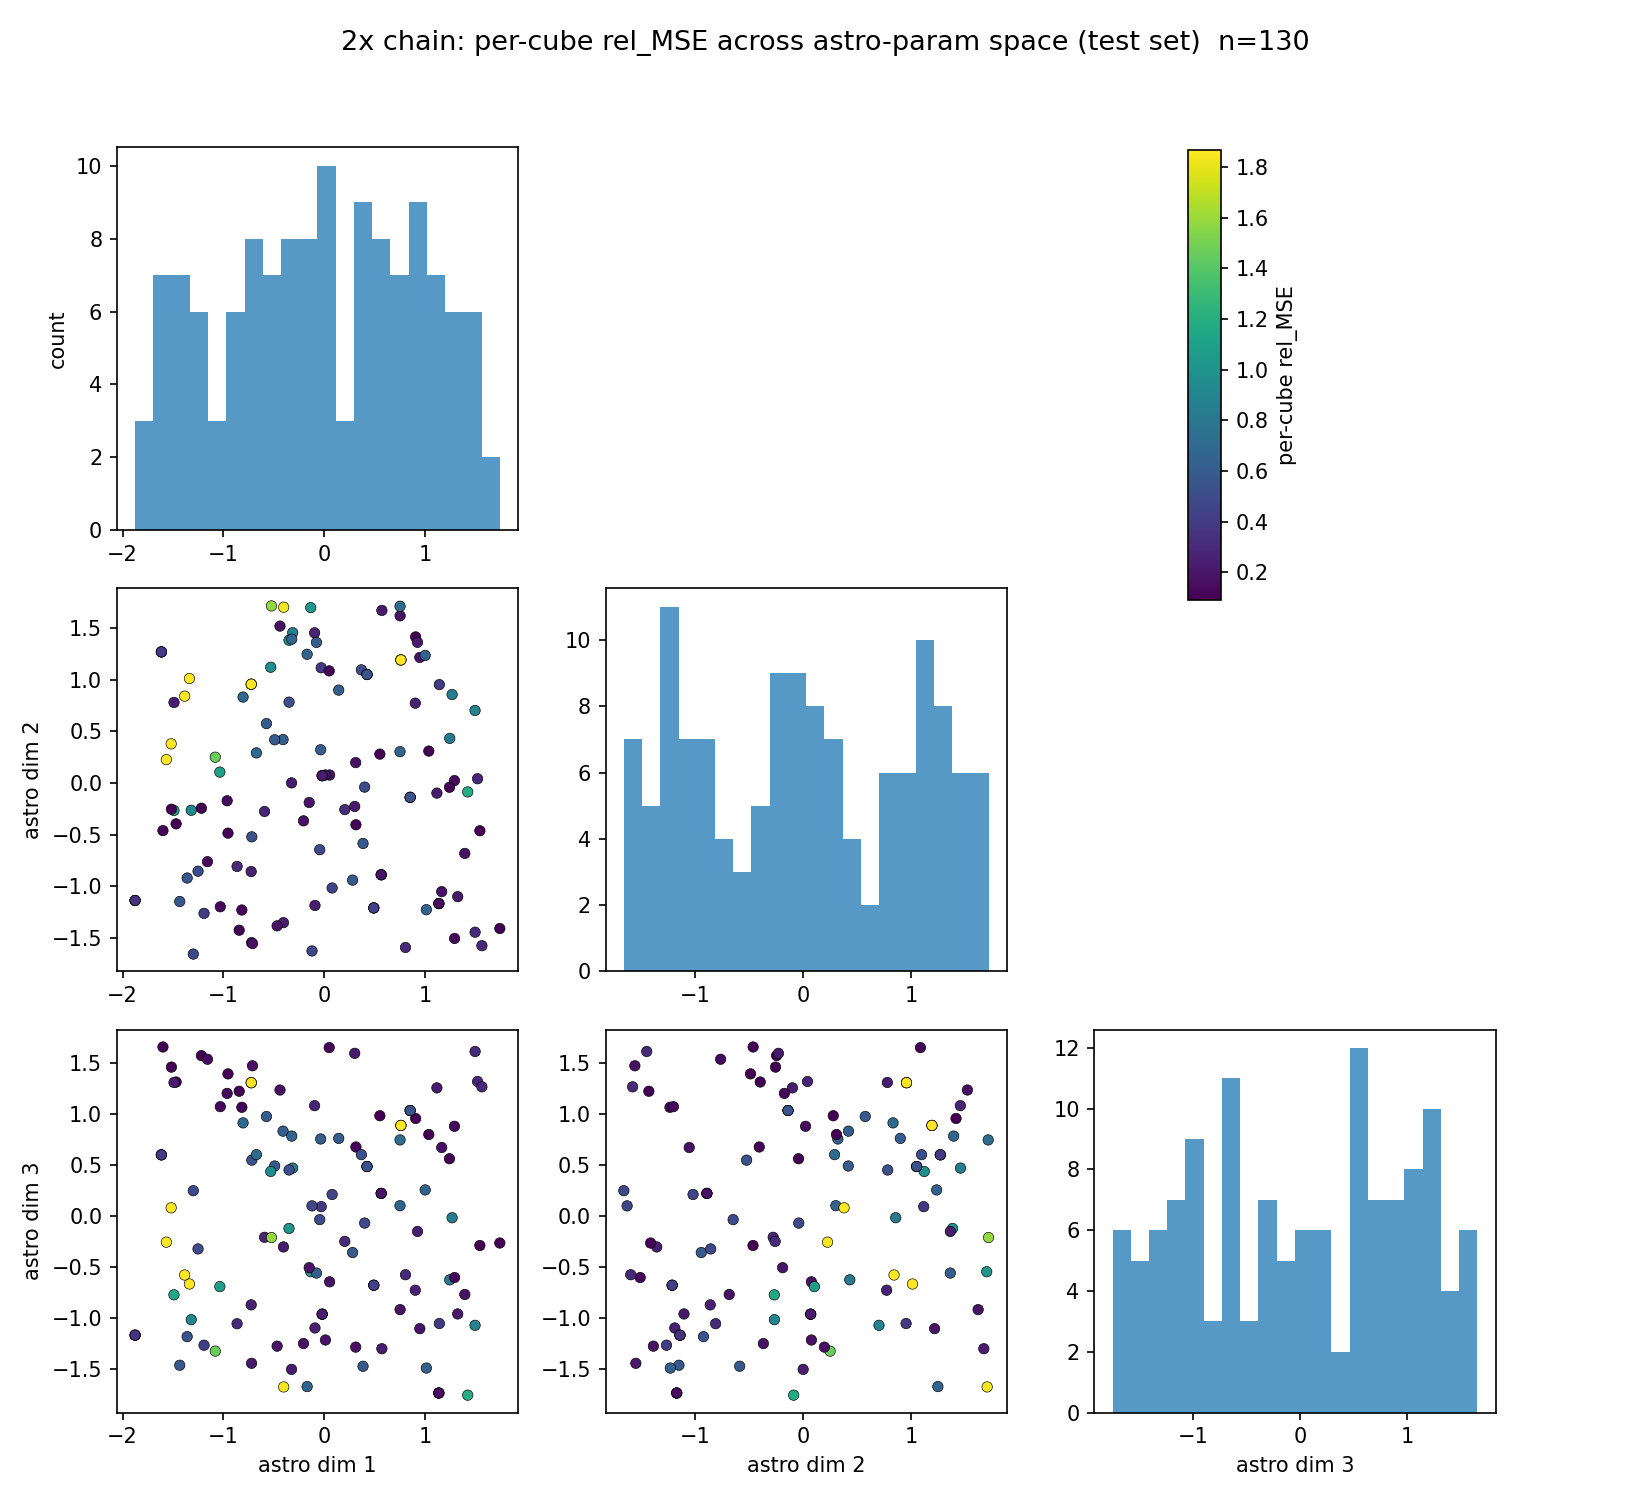
\includegraphics[width=0.75\linewidth]{figures/10_astro_corner_2x.png}
\caption{2$\times$ chain: per-cube $\relMSE$ across the three astrophysical
parameter dimensions of the \texttt{varying\_astro} suite (standardised units;
the fourth parameter recorded is the redshift, and the fifth is the constant
suite indicator, both omitted here).  Bright points are hard cubes; they
cluster in a corner of the parameter space (high ``astro dim 2'', which encodes
the strong-heating / late-reionisation regime), reproducing the pattern
identified for the v1 model in earlier work.  This gives a concrete diagnosis of
where the LDM is undertrained.}
\label{fig:corner}
\end{figure}

\section{Best- and worst-cube inspection}
\label{sec:bestworst}

For the 2$\times$ chain, we show the cubes with the smallest and largest
$\relMSEf$ side-by-side (Fig.~\ref{fig:bw2x}).  With the corrected metric
the ``best'' cube (top, $\relMSEf\!=\!0.36$, $z\!=\!10$) is genuinely
well-reconstructed: the true and generated slices share the same colour
palette, the PDFs largely overlap, and $P(k)$ tracks within a factor of two.
The ``worst'' cube ($\relMSEf\!=\!17$, $z\!=\!7$) is a hard failure mode at an
out-of-distribution redshift where the true field is highly saturated (values
clustered near $0.9$) and the model produces a completely off-scale field,
inflating $P(k)$ by two orders of magnitude.  Analogous plots for 4$\times$,
8$\times$ and 16$\times$ are provided in
\texttt{figures/12\_bestworst\_4x.png} etc.

\begin{figure}[ht]
\centering
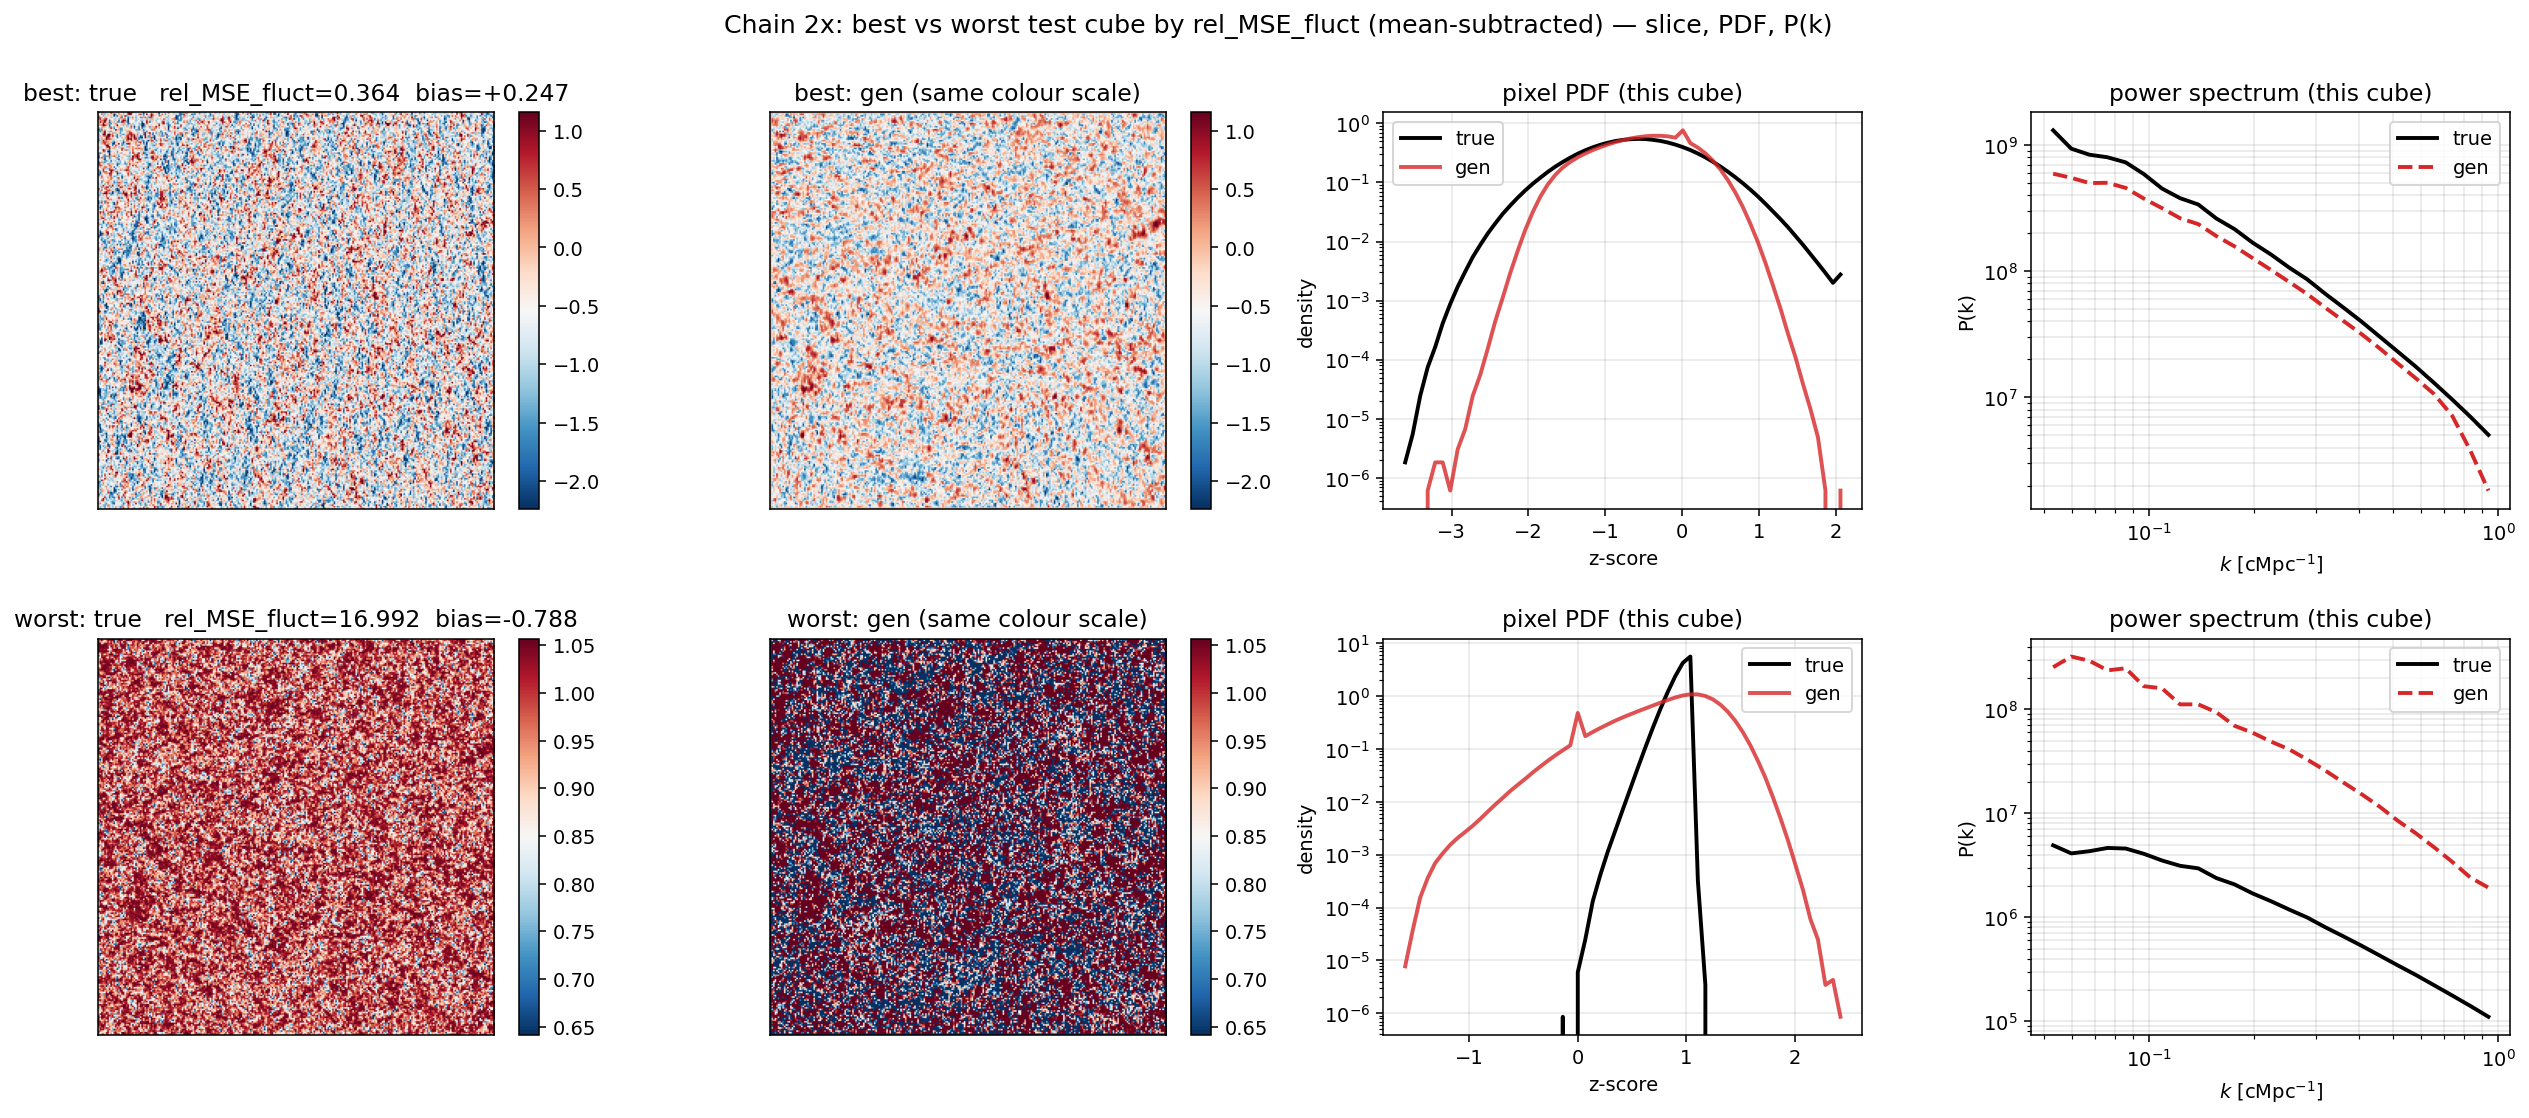
\includegraphics[width=\linewidth]{figures/12_bestworst_2x.png}
\caption{2$\times$ chain: best (top) and worst (bottom) test cubes ranked by
$\relMSEf$ (mean-subtracted).  Columns from left: mid-slice of the true field;
same-scale mid-slice of the generated field; single-cube pixel PDF; single-cube
1-D power spectrum.  The best cube ($z\!=\!10$, in-distribution) is visually
consistent between true and gen; the worst cube ($z\!=\!7$, out-of-distribution,
highly saturated) is a mode-collapse-like failure with $P(k)$ inflated by two
orders of magnitude.}
\label{fig:bw2x}
\end{figure}

\begin{figure}[ht]
\centering
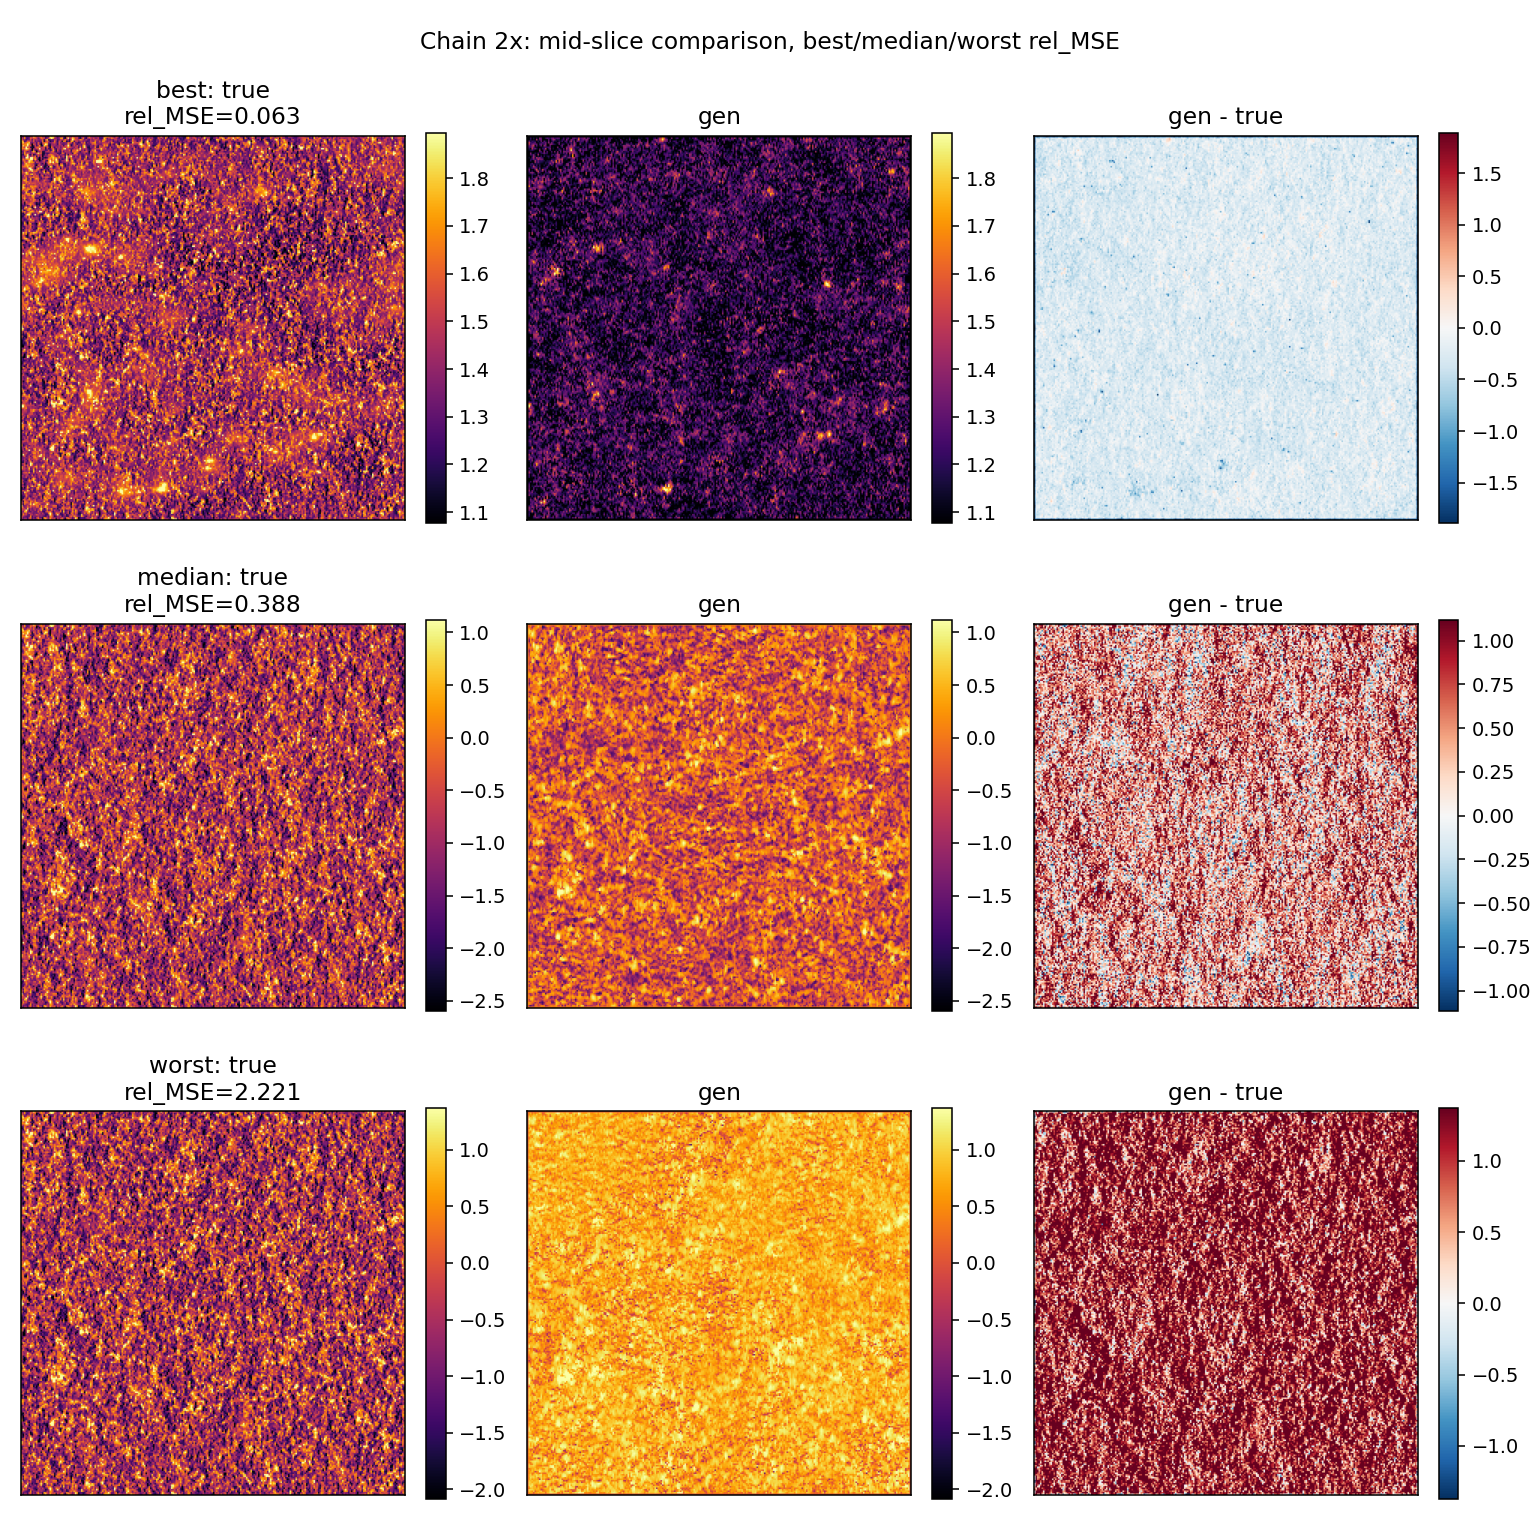
\includegraphics[width=\linewidth]{figures/9_slices_2x.png}
\caption{2$\times$ chain: mid-slice comparisons across best / median / worst
$\relMSE$ cubes.  Columns are: true, gen (same colour scale), and residual
(gen $-$ true).  The best cube shows a small systematic negative residual
(gen is a hair too cold); the median cube shows structured positive residuals
correlated with the true bright regions (the model under-shoots high-amplitude
features); the worst cube shows a global positive bias.  The story is the same
for the other three compression chains --- see
\texttt{figures/9\_slices\_\{4x,8x,16x\}.png} --- with the systematic bias
growing monotonically with compression ratio.}
\label{fig:slices2x}
\end{figure}

\section{Inference cost}
\label{sec:cost}

\begin{figure}[ht]
\centering
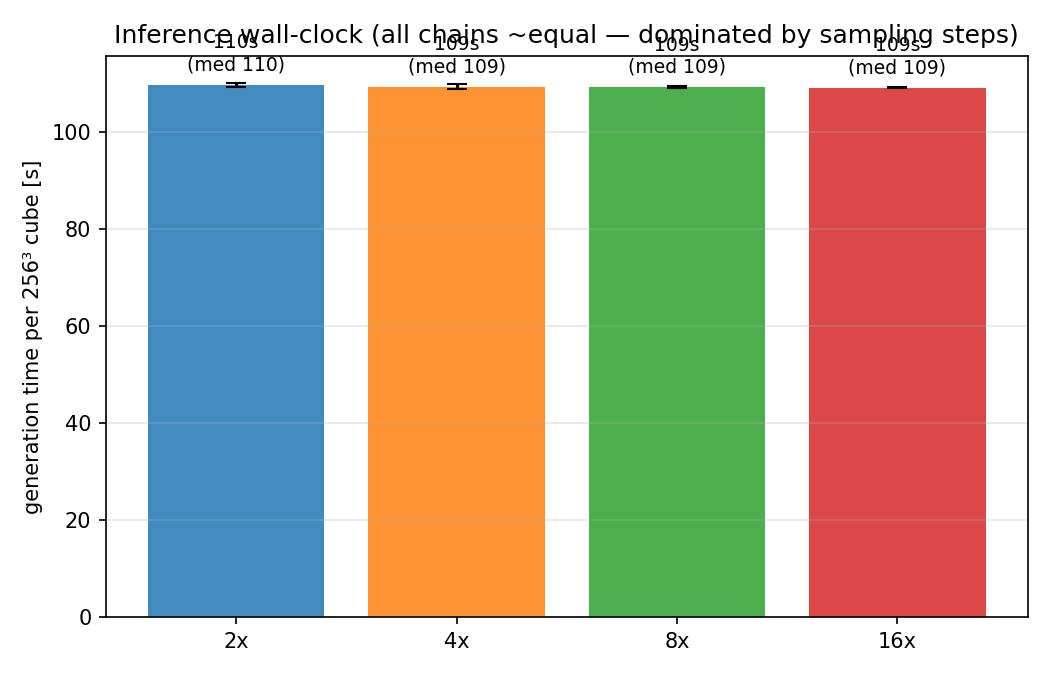
\includegraphics[width=0.7\linewidth]{figures/5_timing_bar.png}
\caption{Wall-clock generation time per $256^3$ cube on an A100 GPU.  The four
chains take essentially the same time ($\sim\!110\,\mathrm{s}/\text{cube}$)
because inference cost is dominated by the number of diffusion sampling steps
(30 Heun steps $\times$ 343 tiles per cube) and by the tile-stitching overhead,
not by the latent tensor size.  Compression ratio therefore buys nothing at
inference time --- its potential savings are entirely in training compute and
memory, and only if the smaller latent still holds enough information.  Given
the results above, the 2$\times$ chain is the strict-Pareto-dominant choice.}
\label{fig:timing}
\end{figure}

\section{Conclusion and next steps}
\label{sec:conclusion}

Across every physically-relevant statistic --- power spectrum, bispectrum,
cross-coherence, pixel PDF and variance --- the \textbf{2$\times$ chain
(latent channels = 32) is the only paper-grade candidate}, while pixel MSE
alone would have selected 4$\times$ for the wrong reason.  Higher-compression
chains lose small-scale power, under-represent the emission tail of the pixel
PDF and inflate the bispectrum; the loss grows monotonically with compression
ratio.  Because all four chains have identical inference wall-clock, there is
no efficiency argument for the more-compressed chains at deployment.

Recommended next steps:
\begin{itemize}
  \item Train the conditional-residual network on top of 2$\times$ to recover
        the remaining $k\!>\!0.5\,\Mpc$ power loss and the exaggerated
        small-scale bispectrum.  Higher-compression chains are not worth
        residual polishing because the residual would have to invent the
        missing 25--40\,\% of the total power, not merely correct the tail.
  \item Fix the \texttt{edm\_precond(\ldots, sigma\_data)} duplicated-kwarg
        crash in \texttt{train\_ldm\_joint\_finetune.py} and rerun the joint
        LDM$+$decoder finetune for the 2$\times$ chain (VAE decoder unfrozen,
        40\,\% of the training data refreshed every 5 epochs plus the entire
        validation set).
  \item Diagnose the ``uniform-field'' worst-cube failure at $z\!=\!9$
        (Fig.~\ref{fig:bw2x} bottom): investigate whether the CFG scale or
        the IC-conditioning strength drops the model into a degenerate mode.
\end{itemize}

\end{document}
